\chapter{Prozess Architekturplanung}
\section{Erstellen der Minimalen Architektur}
Das Kontext Diagramm, welches im Anforderungsprozess erstellt worden ist, zeigt das System mit allen Akteuren und Nachbarsystemen. Aufbauend darauf kann nun die minimale Architektur erstellt werden, welche sich aus dem System und den Nachbarsystemen ableitet.

\begin{figure}[!htbp]
    \centering
    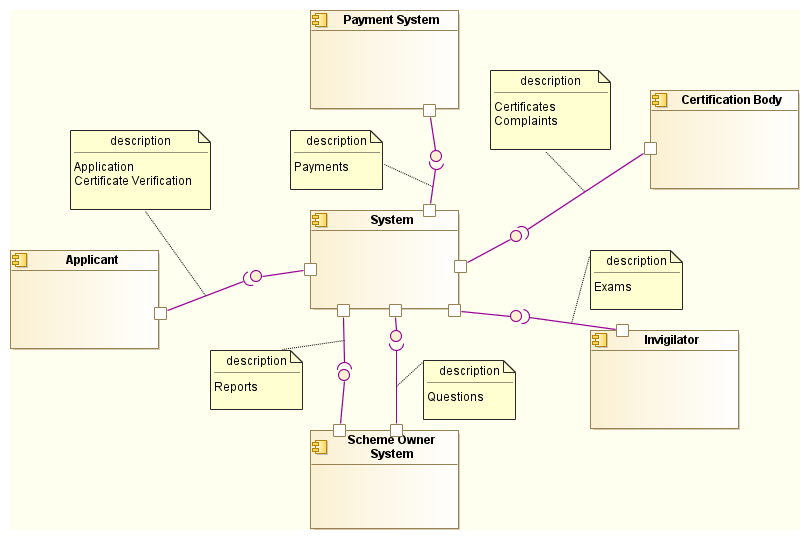
\includegraphics[scale=0.5]{uml/context.png}
    \caption{Das Context Diagramm zeigt das System, die Akteure und die Nachbarsysteme}
\end{figure}

Zuerst werden alle Datenflussnotizen entfernt, danach alle Komponenten, welche kein System darstellen. In diesem Falle werden folgende Komponenten entfernt:

\begin{itemize}
  \item Applicant
  \item Certification Body
  \item Invigilator
\end{itemize}

Dies führt zu folgender Minimalarchitektur:

\begin{figure}[!htbp]
    \centering
    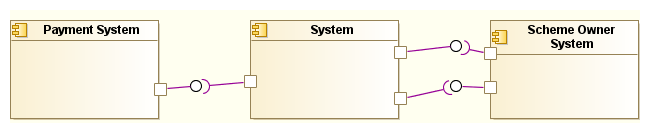
\includegraphics[scale=0.5]{uml/minimalarch.png}
    \caption{Minimale Architektur}
\end{figure}

Für die Nachbarsysteme wird keine Architektur erstellt, jedoch beinflussen sie die Schnittstellen des Systemes und sind deswegen wichtig für den weiteren Prozes. Sie werden in die Architektur einbezogen.

\section{Erstellen der Datenminimalarchitektur}
Einteilen der Systeme in Vertrautheitslevel und mit Gateways trennen. Datenflüsse fix vorgeben (darf keinen Gateway überspringen). Erklären was die Gateways machen und warum sie gut skalierien

Warum aufspalten? Problem bei Zugriff auf gleiches system, überlegung: jeder akteur kann sicherheitslücken ausnutzen um system zu knacken und andere daten zu lesen/manipulieren. außerdem möchte man das system so weit wie möglich absichern und nur die benötigten sachen erlauben. je mehr sachen auf dem system gemacht wird, desto mehr muss erlaubt werden und desto anfälliger ist das system

Wieviele level gibt es? Vertrautheitshirarchie muss aufgebaut werden, manchmal gibt es paralelle systeme (zb internal könnte in mehrere Abteilungen aufgeteilt werden, diese könnten wiederum unterschiedliche vertraute level haben) Grundidee ist die Zugriffsregelung, so wenig unterschiedliche kontrollinstanzen/firewalls wie möglich zu verwenden, damit weniger wartungsaufwand ist und weniger fehler passieren können.

\section{Akteuraufteilung nach Vertrautheitslevel}
Definieren wer hat Zugriff auf welche Daten (RW). Kann in einer Matrix dargestellt werden. Daten davon können aus den Objektflüssen des Aktivitätsdiagrammes abgelesen werden


\section{Einbeziehen der Akteure}
Trennen von Akteursystemen basierend auf Daten und Vertrautheitslevel

\section{Modellieren der Komponenten Interfaces (Klassen Diagramm)}
Aufzeigen dass zb das interne System user anlegen können muss mit methoden im klassendiagramm

\section{Analyse der nicht funktionalen Attribute}
Auf Basis von dokumentierten Szenarien können nun nicht funktionale Attribute gemessen werden und Hinweise kritische/wichtige Komponenten gegeben werden. Kostengegenüberstellung können auch eigene Systeme rechtfertigen/entfernen

\subsection{Reliability}
Single Point of Failure Analyse (Matrix Komponente x Usecase), Erklären wie man auf Matrix kommt (Aktivitätsdiagramm), Ausfallskosten (inkl. Wachstumsszenarien)

Einfache Methode zur schätzung der Ausfallkosten, aufzeigen wie durch Reduzieren der Ausfallswahrscheinlichkeit Kosten sinken aber auch Investitionskosten verursachen. Wachstumsszenarien auch einbeziehen in die Rechnung
\subsection{Usability}
In diesem Teil des Prozesses nicht wichtig, da noch keine Implementierung vorhanden.

\subsection{Efficiency}
Efficiency kann pro usecase gemessen werden, zb für antwortzeiten indem man zb die swimlanewechsel der Aktivitätsdiagramme zählt und mit einer konstanten multipliziert (geschätzte Netzwerkgeschwindigkeit). Ansonsten ist es durch die fehlende Implementation nicht möglich die Geschwindigkeit oder den Arbeitsspeicherverbrauch zu messen.

\subsection{Maintainability}
Auslesbar aus der Usecase Matrix, als Summe aller subsysteme,

\subsection{Portability}
In diesem Teil des Prozesses nicht wichtig, da noch keine Implementierung vorhanden.
